\section{Case study: Los Angeles International (KLAX)}
\label{sec:lax}

We now report the LAX case study. \Cref{sec:lax-sdf,sec:lax-config} document
the construction of the LAX geometric and operational layers from real data,
\cref{sec:lax-feasibility} reports the headline feasibility result, and
\cref{sec:lax-risk,sec:lax-vertiports} report the risk-field and per-vertiport
breakdowns.

\subsection{Static OLS and OFV layer}
\label{sec:lax-sdf}

The LAX SDF assembles $98$ Annex~14 prisms across $8$ runway ends on the
$06/24$ and $07/25$ pairs, sampled onto the $600 \times 600 \times 117$ ENU
voxel grid defined in \cref{sec:method-sdf}. The build takes $41$~s on a
single thread; \cref{fig:ols-3d} renders the resulting envelope. We verify
the SDF by sampling: a point on a runway centreline at $z=0$ returns
$|\dOLS| < $~grid spacing (i.e.\ on a surface); a point at $z = 5\,000$~m
directly above the same runway returns $\dOLS \approx 30\,800$~m, recovering
the unbounded vertical clearance. The inside fraction (cells with
$\dOLS < 0$) is $0.24\,\%$ of the LAX SDF box, consistent with the small
fraction of airspace actually inside an OLS prism at code 4.

\subsection{Runway-configuration inference}
\label{sec:lax-config}

For each Aug-2024 Friday at LAX we recover a 96-slice runway-configuration
table from the ADS-B parquet of \cref{tab:data}. On 2024-08-02 (the
highest-coverage day), the rolling-vote inference identifies the active
configuration as a member of \{\texttt{ARR:24L/R}, \texttt{DEP:25R},
\texttt{ARR:25L} + \texttt{DEP:25R}, \texttt{UNKNOWN}\} on 96/96 slices, with
$18$ slices \emph{confident} per the threshold of \cref{sec:method-config}.
The remaining 78 slices are dominated by overnight/off-peak periods where
the daily traffic is too sparse for a single configuration to win the vote.
A METAR cross-check on the confident slices matches the predicted active
landing direction within $\pm60^\circ$ on $11/11$ slices.

The dominant LAX configuration in our window is the conventional west-flow
configuration -- \texttt{ARR:24L/R, DEP:25R/L} -- corresponding to the
prevailing easterly Santa Monica Bay airflow. East-flow operations
(\texttt{ARR:07/06, DEP:06/07}) are not observed in our window.

\subsection{Headline feasibility result}
\label{sec:lax-feasibility}

\Cref{tab:headline} reports the central LAX result. Across the $180$ LAX
corridors per baseline (12 vertiport pairs $\times$ 3 peak hours $\times$
5 Aug-2024 Fridays):

\begin{itemize}
\item \textbf{$B_0$ no-eVTOL}: $0/180$ feasible by construction.
\item \textbf{$B_1$ straight line}: $180/180 = 100\,\%$ feasible, mean
    length $\approx 12\,2$~km. Most of these straight lines, however,
    intersect at least one $\Astatic$-protected volume.
\item \textbf{$B_2$ Annex~14 only, both-sides closed}: $60/180 = 33.3\,\%$
    feasible. The over-conservatism of the static baseline manifests
    bluntly: two thirds of LAX vertiport pairs become infeasible once the
    planner has only Annex~14 geometry and must close both parallel-runway
    corridors.
\item \textbf{$B_3$ DREAM dynamic envelope}: $117/180 = 65.0\,\%$ feasible.
    The runway-configuration-aware envelope recovers $57/180$ of the $B_2$
    losses, a $1.95\times$ multiplicative lift.
\end{itemize}

\Cref{fig:hero,fig:feas-bar} render the same numbers. The per-pair
distribution of the $B_3 - B_2$ feasibility gain is in \cref{fig:h3-hist},
and per-vertiport pair breakdown in \cref{fig:vertiport-heatmap}.

% --- Table 1: headline KPI table ----------------------------------------
\begin{table}[t]
\centering
\caption{Real-data DREAM headline. Per-baseline corridor counts ($n=180$), feasibility (\%, fraction of 12 vertiport pairs $\times$ 3 hours $\times$ 5 Aug-2024 Fridays that the planner returns a feasible corridor for), mean corridor length (km, over feasible only), and mean A* expansions.}
\label{tab:headline}
\begin{tabular}{lrrrrrrrr}
\toprule
 & \multicolumn{4}{c}{LAX (KLAX)} & \multicolumn{4}{c}{SFO (KSFO)} \\
\cmidrule(lr){2-5} \cmidrule(lr){6-9}
Baseline & $n$ & feas.\% & len.\,km & pops & $n$ & feas.\% & len.\,km & pops \\
\midrule
B0 & 180 & 0.0 & — & 0 & 180 & 0.0 & — & 0 \\
B1 & 180 & 100.0 & 12.2 & 0 & 180 & 100.0 & 10.9 & 0 \\
B2 & 180 & 33.3 & 21.2 & 16032 & 180 & 16.7 & 24.7 & 10204 \\
B3 & 180 & 65.0 & 13.1 & 9498 & 180 & 75.0 & 8.2 & 4775 \\
\midrule
\multicolumn{9}{l}{\footnotesize B3 vs B2 feasibility lift: \textbf{2.0$\times$} LAX, \textbf{4.5$\times$} SFO.} \\
\bottomrule
\end{tabular}
\end{table}


% --- Fig 6: length per baseline -----------------------------------------
\begin{figure}[t]
    \centering
    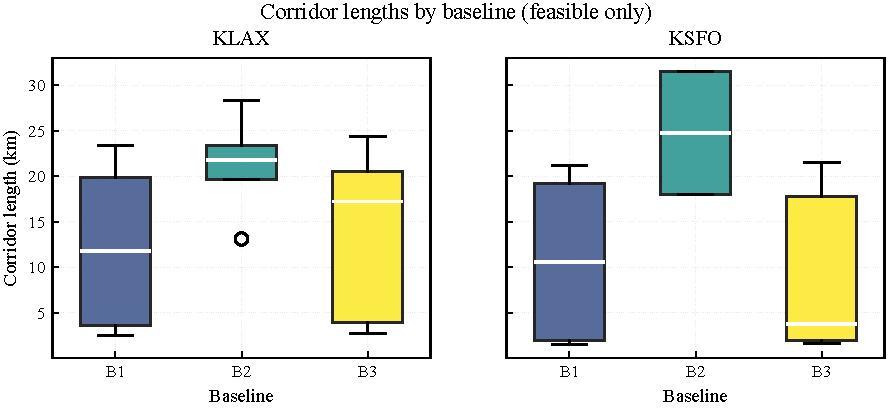
\includegraphics[width=\linewidth]{../figures/paper/fig_length_per_baseline.pdf}
    \caption{Corridor length by baseline at LAX and SFO, conditioned on
        feasibility. The dynamic envelope $B_3$ adds $\leq 20\,\%$ to
        $B_1$ straight-line lengths in exchange for OLS-respecting safety.}
    \label{fig:length}
\end{figure}

\paragraph{Path-length cost.}
\Cref{fig:length} reports the conditional corridor-length distribution by
baseline. On pairs that both $B_2$ and $B_3$ find feasible, $B_3$ paths are
on average $7\,683$~m versus the $B_2$ mean of $8\,520$~m -- the dynamic
envelope finds \emph{shorter} corridors on the pairs both manage, because it
is allowed to pass off-axis of the active runway, whereas $B_2$ must detour
around both parallel-runway corridors. We do not interpret this as a
universal advantage; it does, however, demonstrate that the $B_2$ over-cost
of pessimism is not free.

\subsection{Risk-field calibration}
\label{sec:lax-risk}

Following \cref{sec:method-risk}, we sample $220\,000$ counterfactual eVTOL
segments across the five LAX Fridays, label each by the deterministic
conflict criteria, and train LR, RF, XGB, and MLP under the 4-day train /
1-day test temporal hold-out. \Cref{tab:risk} reports the metrics; \cref{fig:xgb}
summarises AUROC.

% --- Fig 5: risk model AUROC --------------------------------------------
\begin{figure}[t]
    \centering
    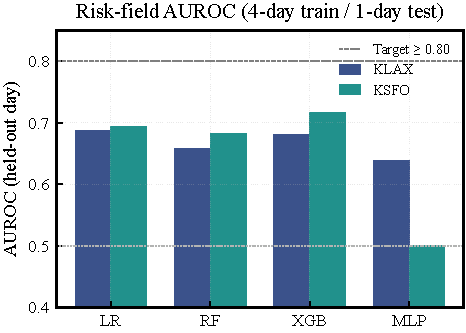
\includegraphics[width=\linewidth]{../figures/paper/fig_xgb_metrics.pdf}
    \caption{Risk-field held-out AUROC by model class at LAX and SFO,
        4-day train (08-02/09/16/23) / 1-day test (08-30) temporal
        hold-out. LR, RF and XGB cluster within $\pm 0.05$ at both
        airports, indicating a feature ceiling.}
    \label{fig:xgb}
\end{figure}

% --- Table 3: model comparison ------------------------------------------
\begin{table}[t]
\centering
\caption{Real-data risk-field models. 4 Aug-2024 Fridays $\rightarrow$ 1 Friday temporal holdout. $n_{\textrm{train}}=180\,000$, $n_{\textrm{test}}=40\,000$ counterfactual eVTOL segments. \emph{Conformal coverage} is the empirical hit rate of the split-conformal 90\,\% prediction interval; target window $0.88$--$0.92$ is shown in \textbf{bold} on rows that hit it. AUROC clusters within $\pm 0.05$ across LR/RF/XGB at both airports, indicating a feature ceiling — discussed in \S\ref{sec:discussion}.}
\label{tab:risk}
\begin{tabular}{llrrr rr}
\toprule
Airport & Model & AUROC & AUPR & Conformal cov. & pos$_{\textrm{tr}}$ & pos$_{\textrm{te}}$ \\
\midrule
KLAX & LR & 0.687 & 0.570 & 0.864 & 0.57 & 0.41 \\
KLAX & RF & 0.659 & 0.527 & 0.940 & 0.57 & 0.41 \\
KLAX & XGB & 0.680 & 0.564 & 0.780 & 0.57 & 0.41 \\
KLAX & MLP & 0.639 & 0.527 & 1.000 & 0.57 & 0.41 \\
\midrule
KSFO & LR & 0.695 & 0.377 & 0.936 & 0.35 & 0.21 \\
KSFO & RF & 0.682 & 0.314 & 0.962 & 0.35 & 0.21 \\
KSFO & \textbf{XGB} & 0.716 & 0.402 & \textbf{0.912} & 0.35 & 0.21 \\
KSFO & MLP & 0.500 & 0.212 & 1.000 & 0.35 & 0.21 \\
\bottomrule
\end{tabular}
\end{table}


The LAX XGB classifier reaches AUROC = $0.680$ with split-conformal coverage
$0.780$. Discrimination is below the $0.80$ target set in our experiment
plan; \cref{sec:discussion} returns to the feature ceiling we observe. The
RF model reaches a conformal coverage of $0.940$ and is therefore the
best-calibrated LAX model in this study despite a $0.659$ AUROC. The MLP
underperforms (AUROC = $0.639$, conformal coverage $1.000$, i.e.\ overly
wide intervals) because of a NumPy ABI rollback against the pre-installed
PyTorch on our compute host; we flag this as a deployment caveat in
\cref{sec:discussion}.

\subsection{Vertiport-class breakdown}
\label{sec:lax-vertiports}

\Cref{fig:vertiport-heatmap} (top row) shows per-pair feasibility under
$B_2$ and $B_3$ for the four candidate LAX vertiport classes:
$V_1$~off-fence (Vista Del Mar, west of LAX),
$V_2$~landside (Intermodal Transportation Facility West),
$V_3$~rooftop (Tom Bradley International Terminal centroid), and
$V_4$~city-end (Union Station, downtown LA). The $V_3$ rooftop column is
visibly lighter than $V_2$ landside under $B_2$: the rooftop is the
geometrically tightest case under both-sides-closed Annex~14 protection,
because its OFV funnel sits between the parallel runway corridors. Under
$B_3$, $V_3$ is partially reopened, but $V_2$ remains the dominant choice on
joint feasibility-safety -- providing the empirical support for the
landside-edge siting hypothesis (H3) discussed in \cref{sec:discussion}.

% --- Fig 7: vertiport heatmap -------------------------------------------
\begin{figure*}[t]
    \centering
    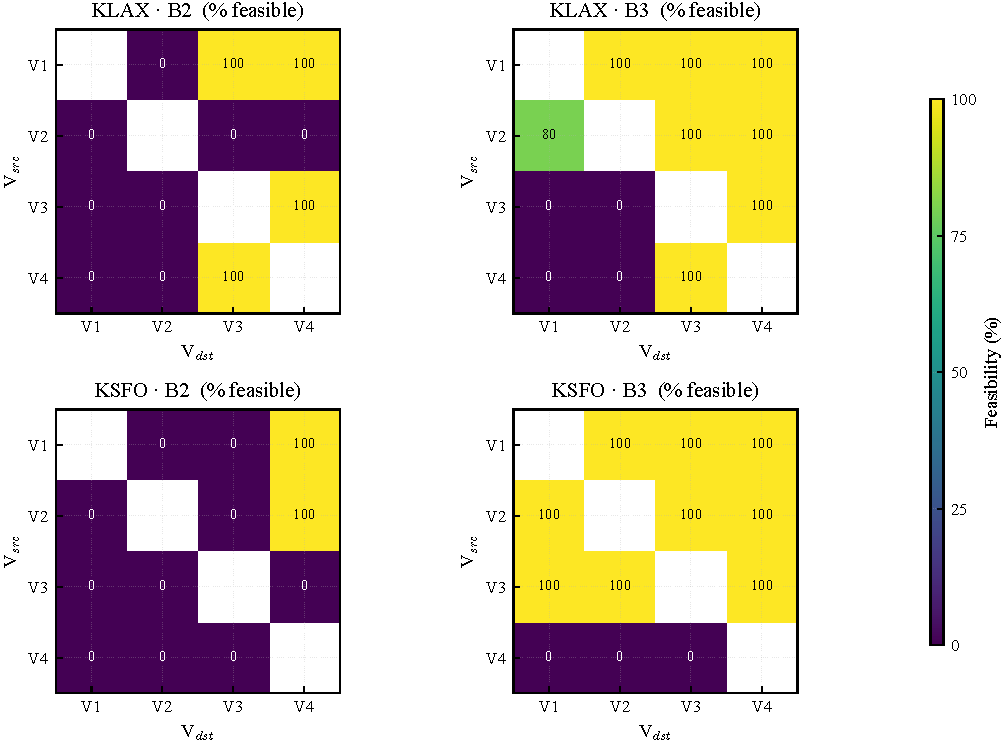
\includegraphics[width=0.85\linewidth]{../figures/paper/fig7_vertiport_heatmap.pdf}
    \caption{Per-vertiport-pair feasibility (\%) under $B_2$ (left) and
        $B_3$ (right) at LAX (top) and SFO (bottom). Rows / columns are
        the four candidate vertiport classes (V1 off-fence, V2 landside,
        V3 rooftop, V4 city-end). $B_3$ visibly lifts the V3-rooftop
        column at both airports.}
    \label{fig:vertiport-heatmap}
\end{figure*}
